\section{System Integration (MPC-H)}
After testing the functioning of both static and dynamic obstacles avoidance together on the sample scenarios, we have proceeded with the integration of the path following task and the obstacle avoidance task. To do so, we have performed the tests with both static and dynamic obstacles exploiting three real scenarios among those already used in the path following tests (Section \ref{chap:path_following}). These tests represent the Model-in-the-Loop, which will be described in detail in Section \ref{subsection:MIL}.
Subsequently, the code has been automatically generated and Software-in-the-Loop tests have been performed (Section \ref{subsection:SIL}). Lastly, the code obtained has been flashed in an evaluation board in order to perform the Processor-in-the-Loop tests (Section \ref{subsection:PIL}).

\subsection{MIL} \label{subsection:MIL}
For the Model-In-the-Loop we have decided to tests our model in three different real scenarios considering the five vehicle models described in Table \ref{tab:vehicle_data}. In particular, the real maps considered are:
\begin{itemize}
    \item Adriatic Highway - A14 : travelled at 100 $km/h$;
    \item Puglia : travelled at 40 $km/h$;
    \item Indianapolis Speedway : travelled at 100 $km/h$.
\end{itemize}
Regarding the obstacles positioning, we have placed them as follows:
\begin{itemize}
    \item Obstacle 1 (static) : placed at 7.5/100 of the total length of the map;
    \item Obstacle 2 (static) : placed at 23/100 of the total length of the map;
    \item Obstacle 3 (static) : placed at 24/100 of the total length of the map;
    \item Obstacle 4 (dynamic) : starting position at 30/100 of the total length of the map in case of the A14 and Puglia scenarios and starting position at 50/100 of the total length of the map in case of Indianapolis (constant speed of 10 $km/h$);
    \item Obstacle 5 (dynamic) : starting position at 36/100 of the total length of the map in case of the A14 and Puglia scenarios and starting position at 56/100 of the total length of the map in case of Indianapolis (constant speed of 20 $km/h$).
\end{itemize}

To integrate the path following test and the dynamic obstacle avoidance test for the MIL phase, we have kept the same assessments on both the path following and the obstacle avoidance tasks, described in Sections \ref{subsection:path_following_testing} and \ref{sub:single_static_obstacle} respectively, resulting in a total of 6 different assessments that have to be verified in order to consider the MIL passed.
In particular, the assessments on the lateral deviation defined for the path following task have been set so that they are taken into account only in Zones 1 and 5. This is due to the fact that, during the overtaking maneuver (Zones 2, 3, and 4), these assessments on the lateral deviation are no longer valid and they are substituted by those used for the obstacle avoidance task.
Figure \ref{fig:mil} shows the overtaking maneuver in the three real maps.
\begin{figure}[H]
\centering

    \begin{subfigure}{.5\textwidth}
    \centering
    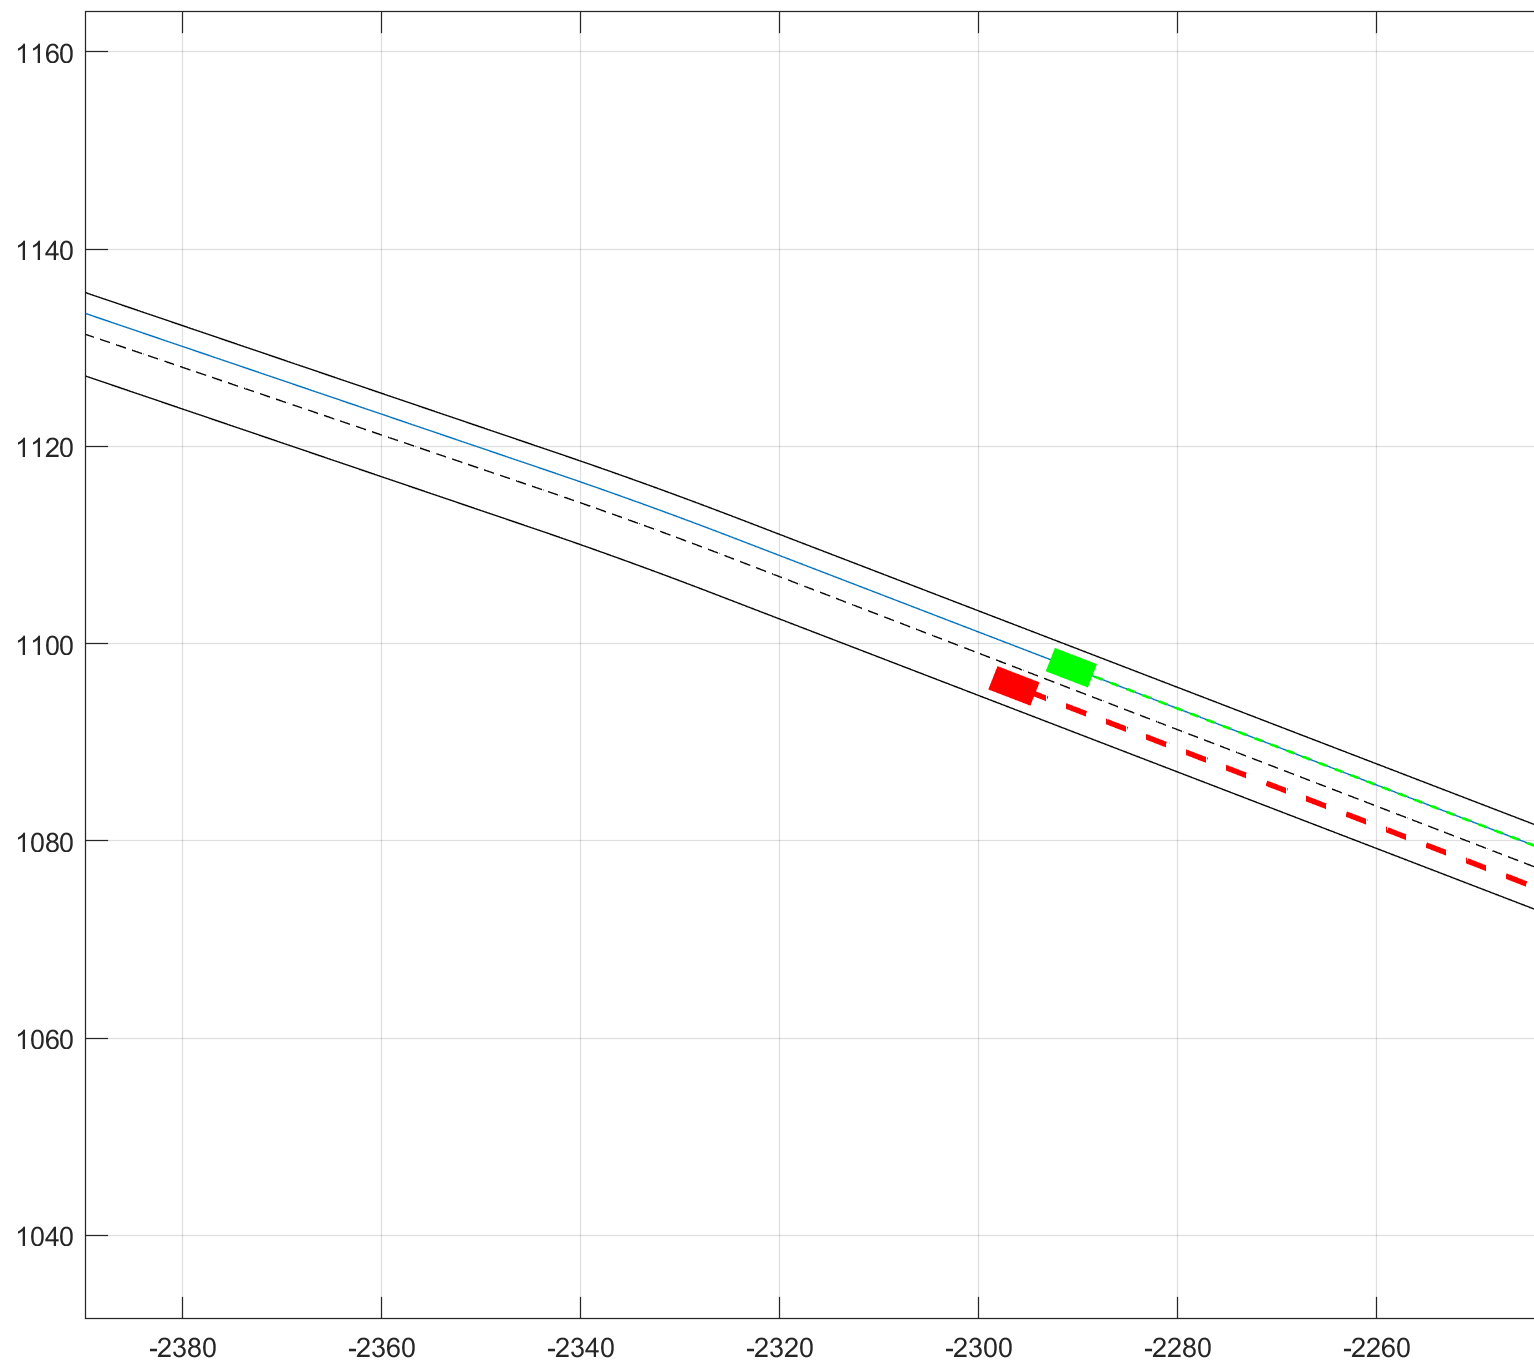
\includegraphics[width=\textwidth,keepaspectratio]{Figures/A_14_green_2.png}
    \caption{Adriatic Highway - A14}
    \label{subfig:a14_mil}
    \end{subfigure}%
    
    \vspace{2mm}
    
    \begin{subfigure}{.5\textwidth}
    \centering
    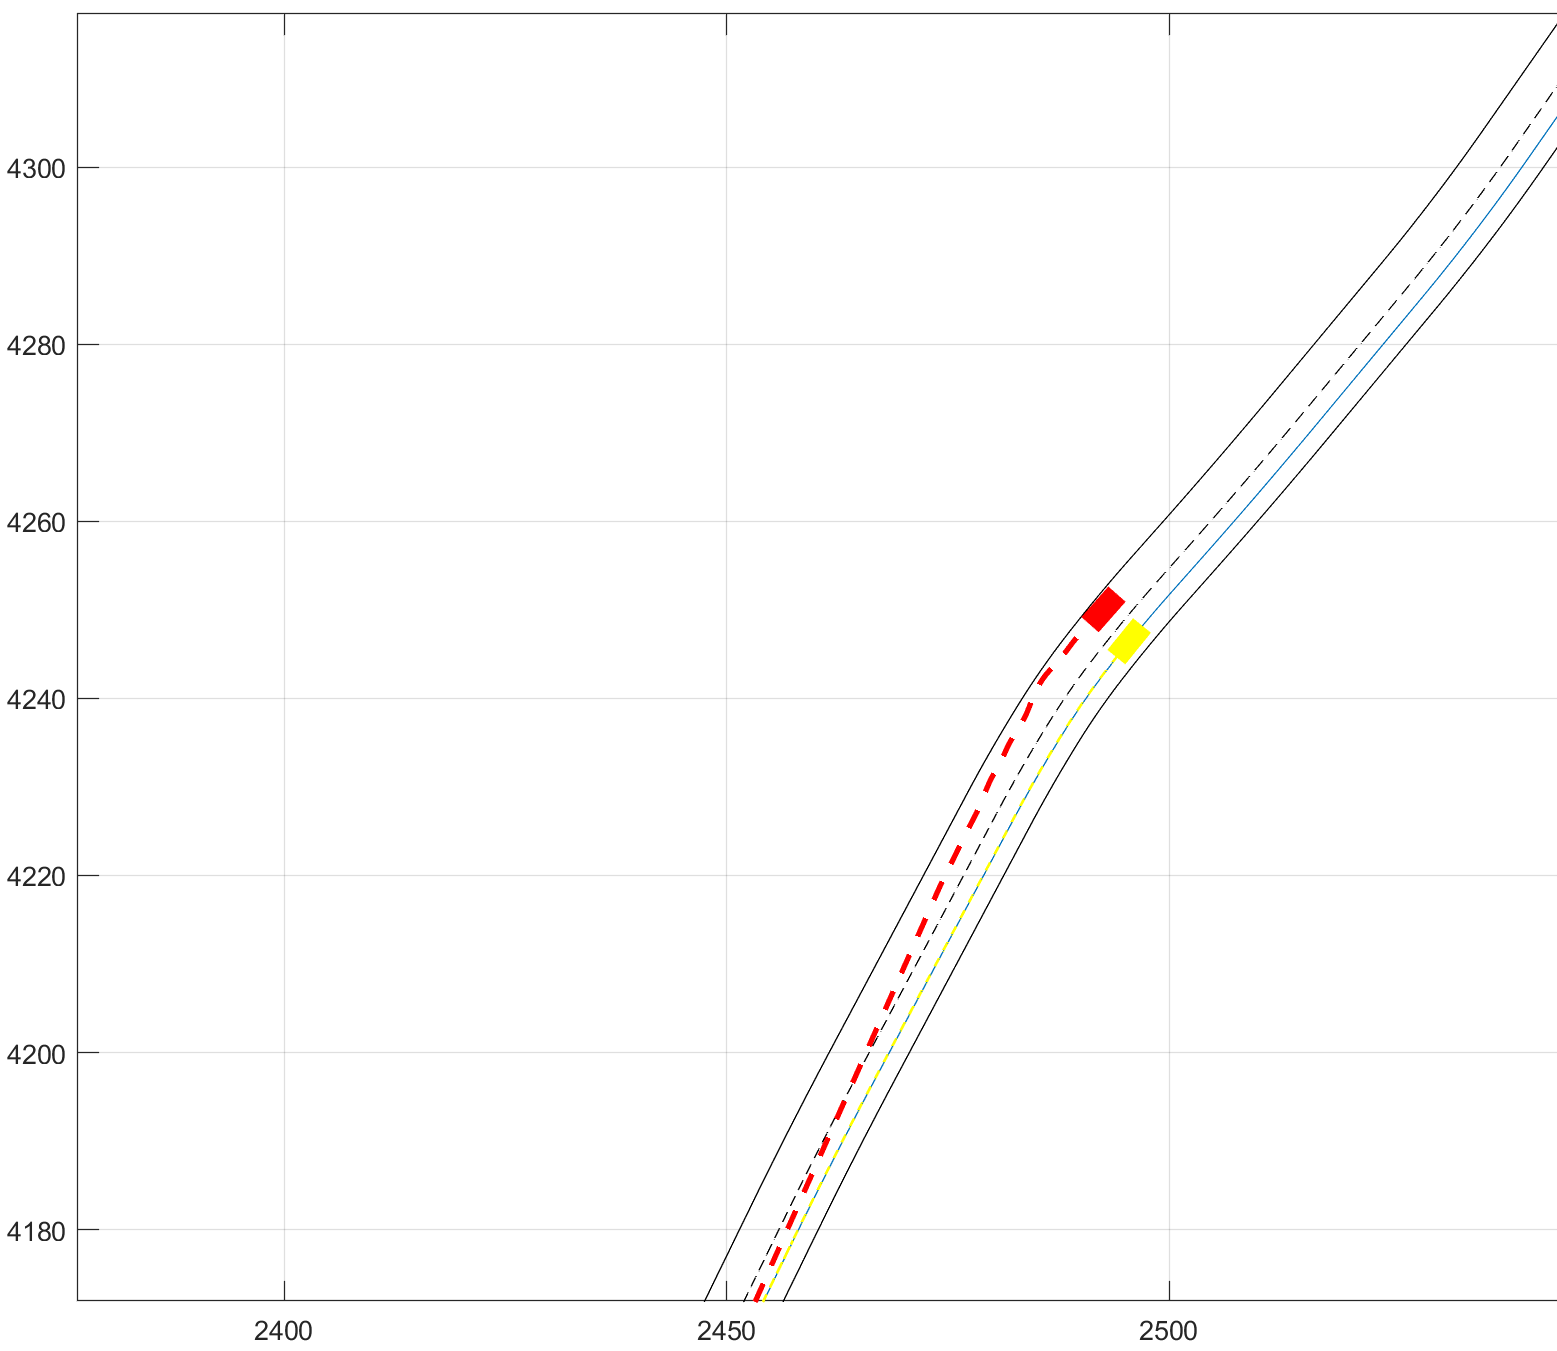
\includegraphics[width=\textwidth,keepaspectratio]{Figures/Puglia_yellow_1.png}
    \caption{Puglia}
    \label{subfig:puglia_mil}
    \end{subfigure}%
    
    \vspace{2mm}
    
    \begin{subfigure}{.5\textwidth}
    \centering
    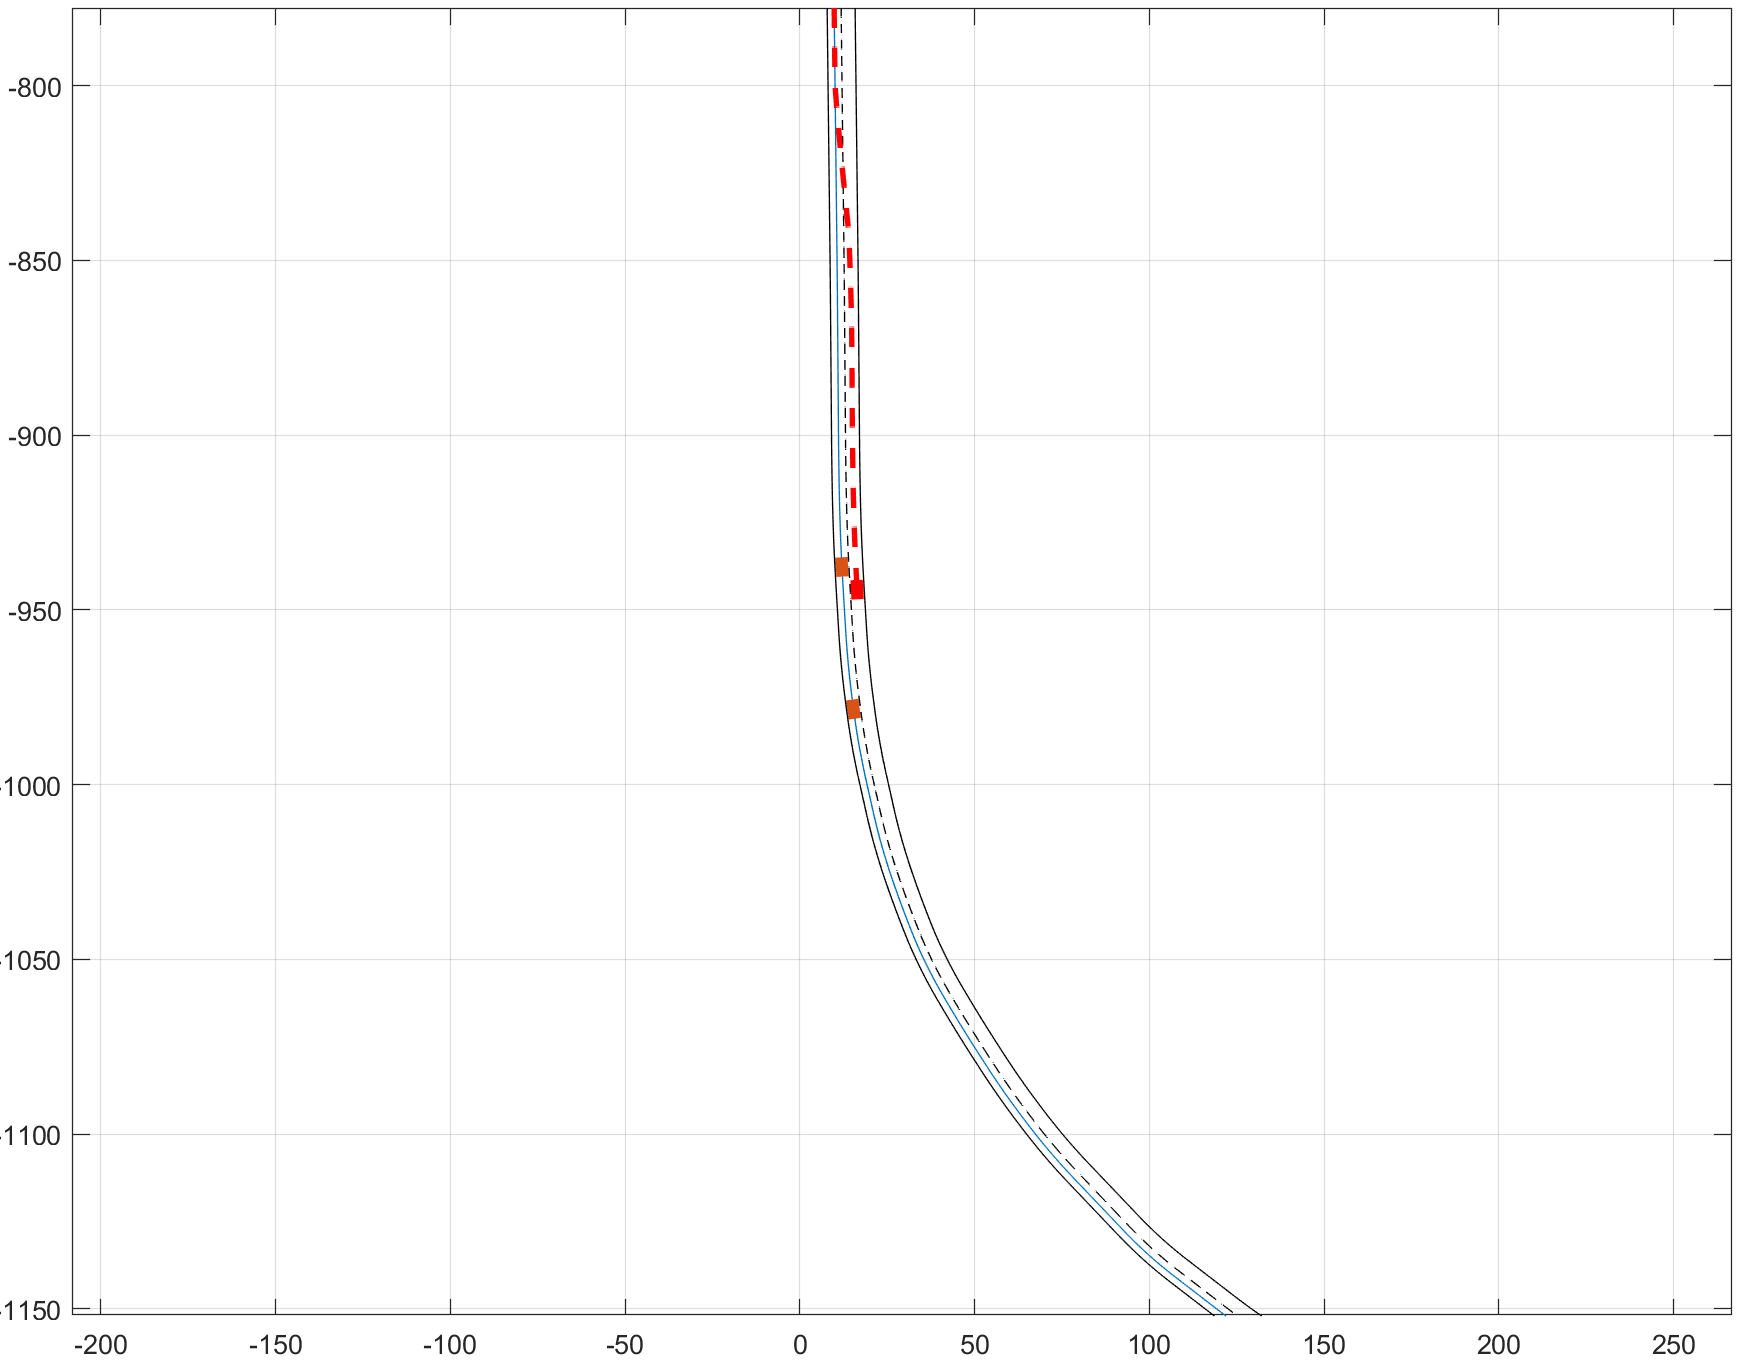
\includegraphics[width=\textwidth,keepaspectratio]{Figures/indianapolis_static_double_2.png}
    \caption{Indianapolis Speedway}
    \label{subfig:indianapolis_mil}
    \end{subfigure}%
    \caption{Snapshots of an overtaking maneuver on each real scenario}
    \label{fig:mil}
\end{figure}

\pagebreak
Further details about the MIL can be found in the documents included in the repository\footnote{The ``Avoidance\_real\_scenarios-test\_report" and ``Avoidance\_real\_scenarios-test\_specification\_report" files generated by Simulink Test are included in the /Documentation/Test Reports/ file path.}.
As it is possible to see in the documents, the model behaved very well without having any failure.

\subsection{SIL} \label{subsection:SIL}

Software-in-the-Loop (SIL) represents the integration of compiled production source code into a mathematical model simulation, providing a practical, virtual simulation environment for the development and testing of our MPC controller. During this phase we have used our PC to test our source code by directly connecting the software to the digital plant model through Simulink.
Thanks to the tool called \textit{Embedded Coder}, which generates readable, compact, and fast C and C++ code for embedded processors \cite{EmbeddedCoder}, we have automatically generated the C code of the SIL block to test its behavior compared to that of the MIL simulation. Indeed, the SIL block is made by the C source code of our MPC controller (see Figure \ref{fig:simulink_mpc}). Before proceeding with the comparison, we have exploited the built-in support for MISRA C software standard contained inside Embedded Coder to check the compliance of the automatically generated code to this standard. The results of this check can be found in the repository\footnote{The ``MISRA-C2012\_Compliance\_Report.html" file generated by Model Advisor is included in the /Documentation/Test Reports/ file path.}.\\

Exploiting Simulink Test, we have created two test harnesses: \textit{Dynamic\_obstacle\_avoidance} and \textit{Dynamic\_obstacle\_avoidance\_SIL}. The former is the complete Simulink model of the system (also used in the tests described in Section \ref{subsection:MIL}) while the latter is the complete system (see Figure \ref{fig:simulink_main}) in which the MPC controller has been substituted by the SIL block. Then, we have executed an Equivalence Test which allowed us to make a comparison between two simulations. In particular, \textit{Dynamic\_obstacle\_avoidance} has been considered as the \textit{baseline} which represent the model simulation output to which our \textit{Dynamic\_obstacle\_avoidance\_SIL} (named \textit{Compare to} in the tests) has been compared in the test in order to verify how they differ. 

In order to compare the behavior of the two simulations we have considered the same three scenarios  together with the six assessments used for the MIL (Section \ref{subsection:MIL}) and we have set different tolerances on the results of both Throttle and Steering Angle (Delta) values of the SIL as reported in Table \ref{tab:SIL_Tolerance}.

\begin{table}[H]
\centering
\begin{tabular}{|l|p{2cm}|}
\hline
\textbf{Steering Angle Relative Tolerance}                        & 1\% \\ \hline
\textbf{Steering Angle Absolute Tolerance {[}rad{]}}              & 0.2 \\ \hline
\textbf{Throttle Relative Tolerance}                              & 1\% \\ \hline
\textbf{Throttle Absolute Tolerance {[}m/s\textsuperscript2{]}} & 2   \\ \hline
\end{tabular}



\caption{SIL relative and absolute tolerances}
\label{tab:SIL_Tolerance}
\end{table}

We have decided to apply these tolerances to the output just to have a meter to compare the two systems in an automatic way.

\pagebreak

Further details about the SIL can be found in the documents included in the repository\footnote{The ``SIL-Test\_Report" and ``SIL-Test\_Specification\_Report" files generated by Simulink Test are included in the /Documentation/Test Reports/ file path.}. 
The Equivalence Test shows good performance of our simulated code in both Adriatic Highway - A14 and Indianapolis Speedway scenarios for all the vehicles, while we have encountered some deviations from the simulated model with the Throttle value in Puglia. These deviations appeared for the Hyundai Azera, Ford E150 and Volkswagen Beetle, while the BMW 325i and the Suzuki Samurai code simulations performed well even in Puglia. In the figures below it is possible to notice the only 3 tolerance failures.

    \begin{figure}[H]
    \centering
    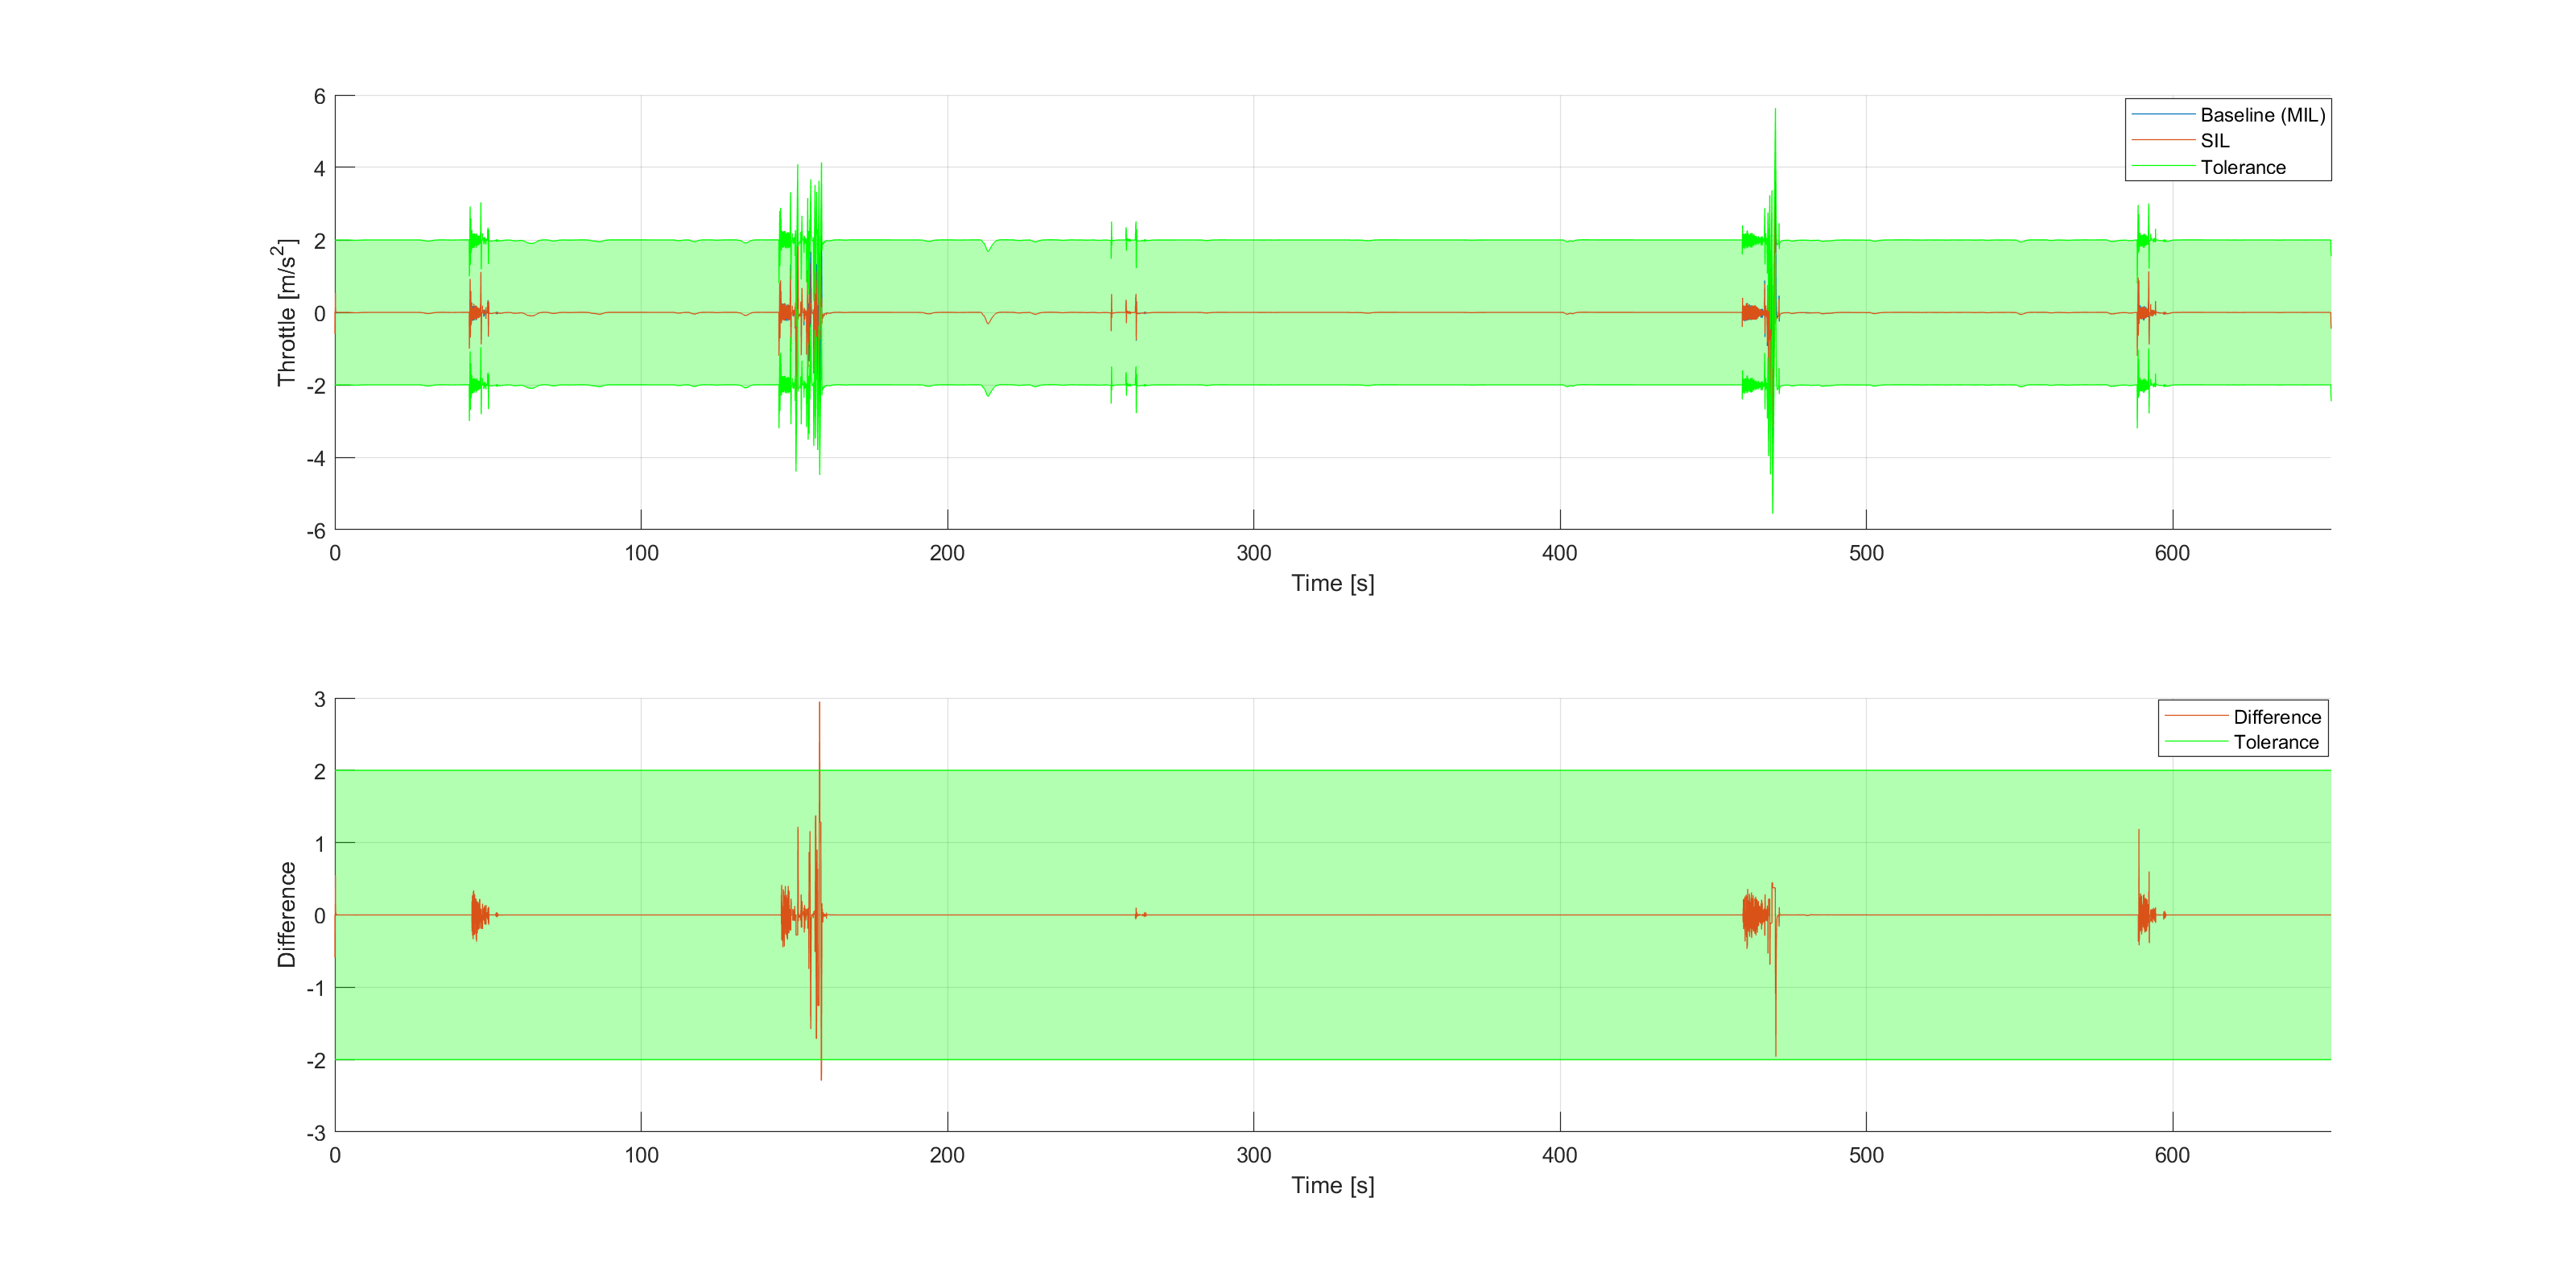
\includegraphics[width=1.1\textwidth,keepaspectratio]{Figures/throttle_azera.png}
    \caption{Throttle deviations with Hyundai Azera in Puglia}
    \label{fig:throttle_azera}
    \end{figure}%
    
    \begin{figure}[H]
    \centering
    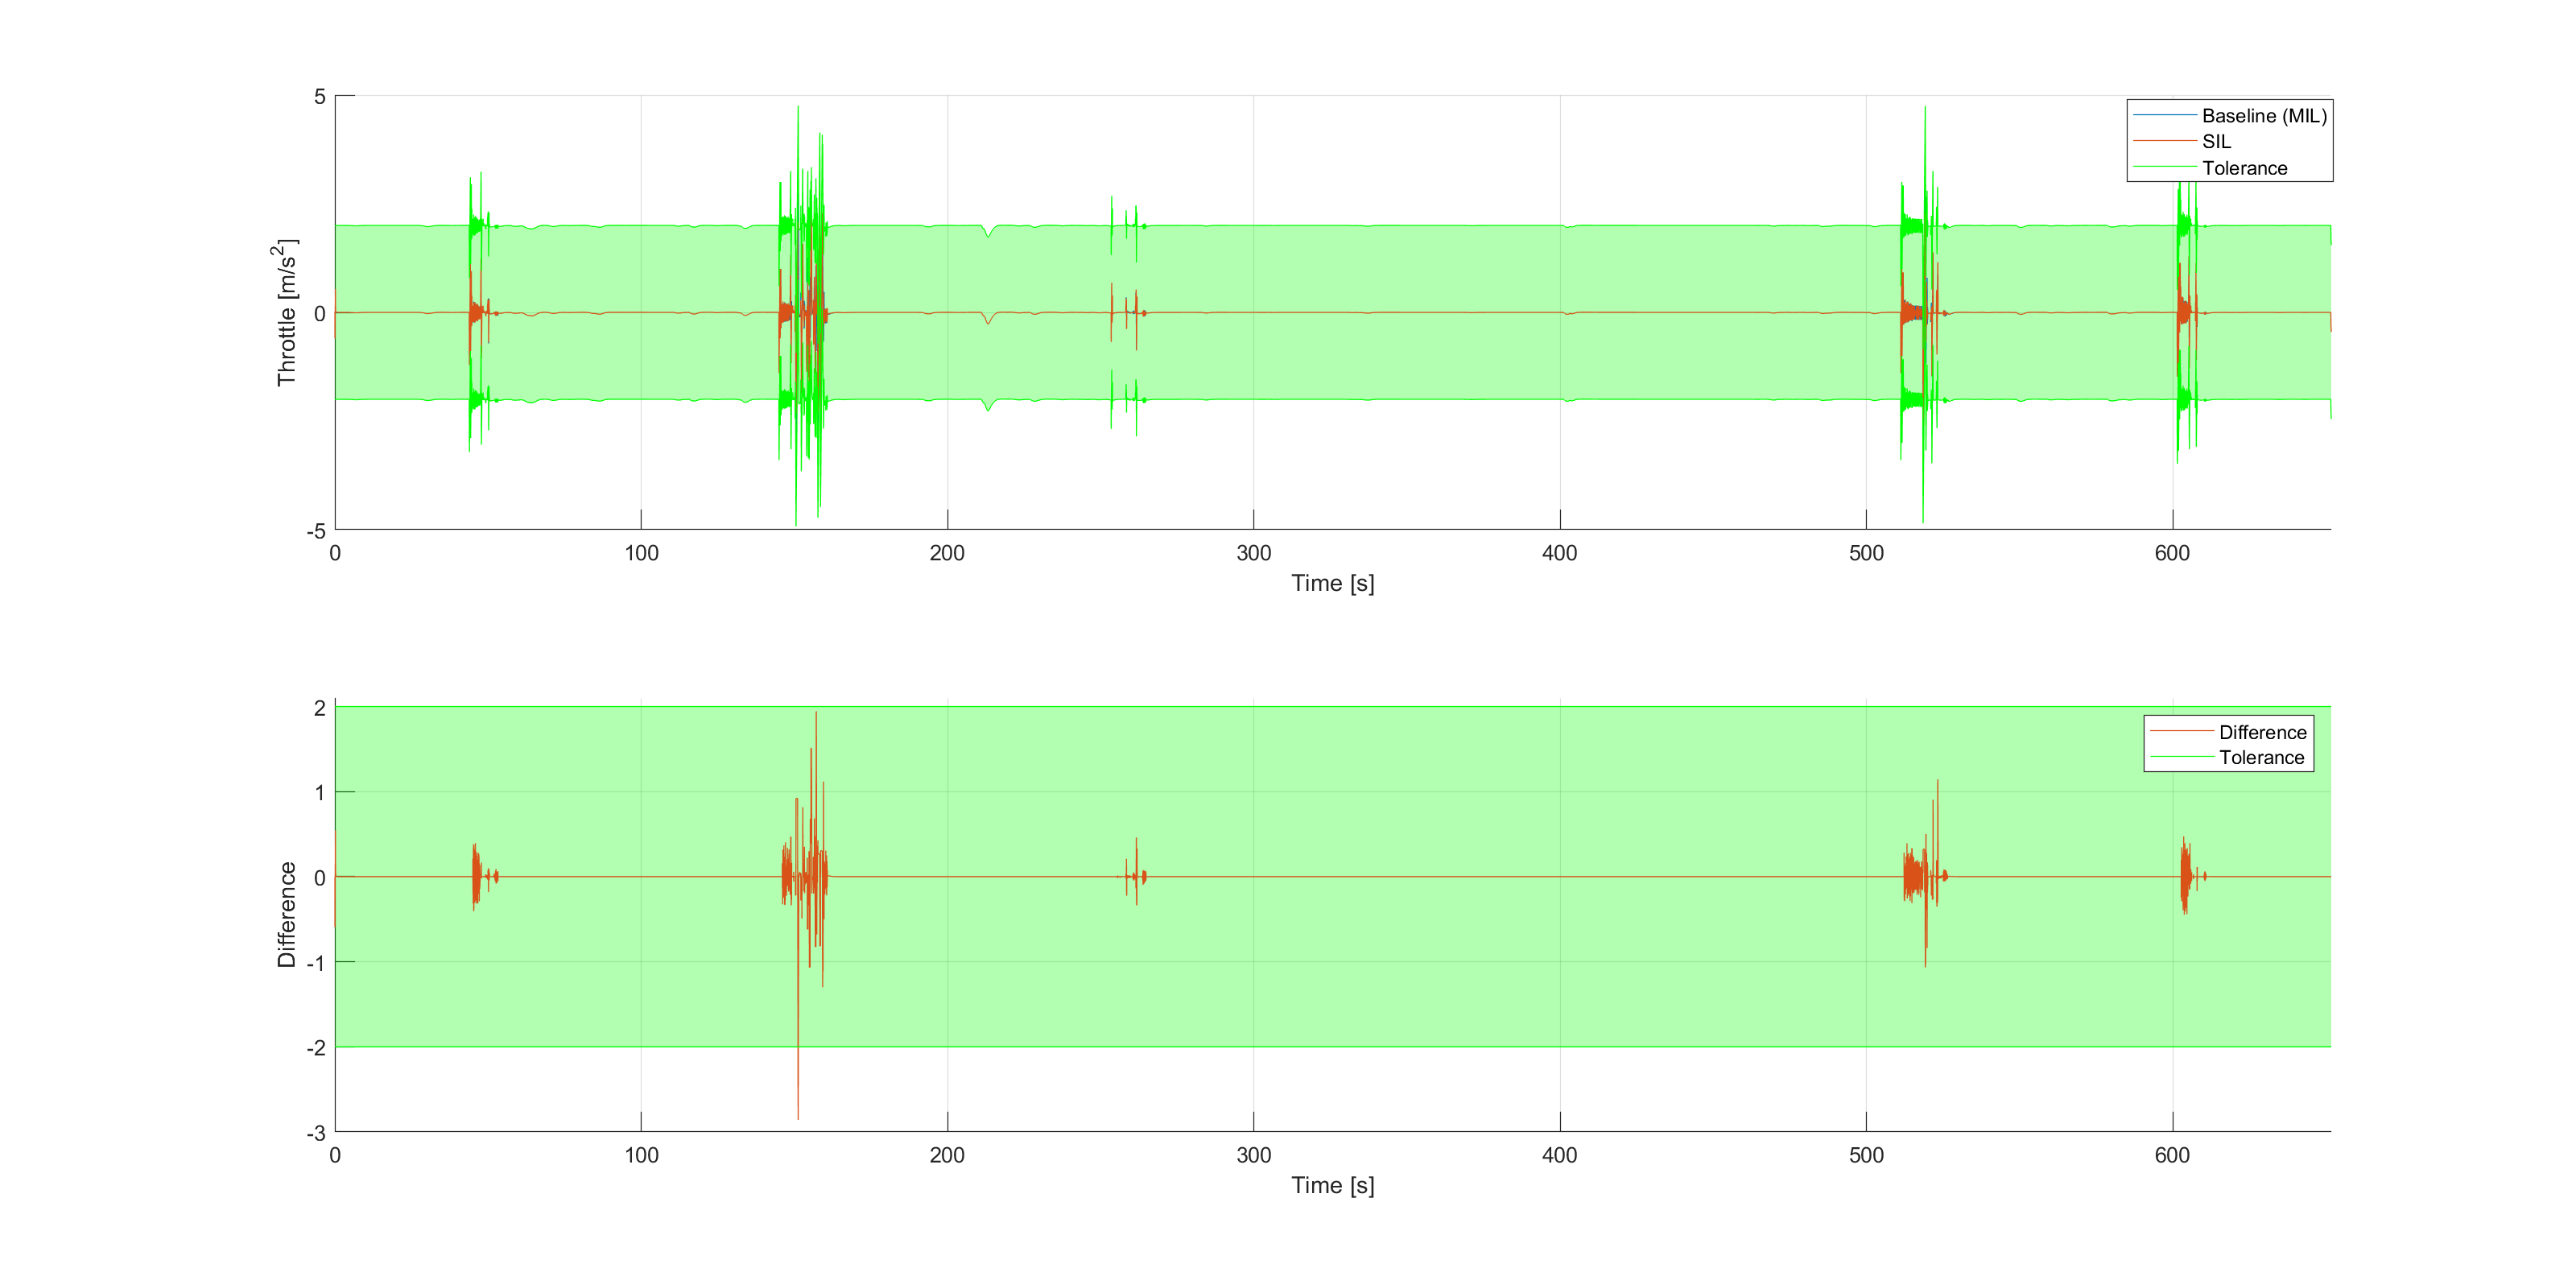
\includegraphics[width=1.1\textwidth,keepaspectratio]{Figures/throttle_ford.png}
    \caption{Throttle deviations with Ford E150 in Puglia}
    \label{fig:throttle_ford}
    \end{figure}%
    
    \begin{figure}[H]
    \centering
    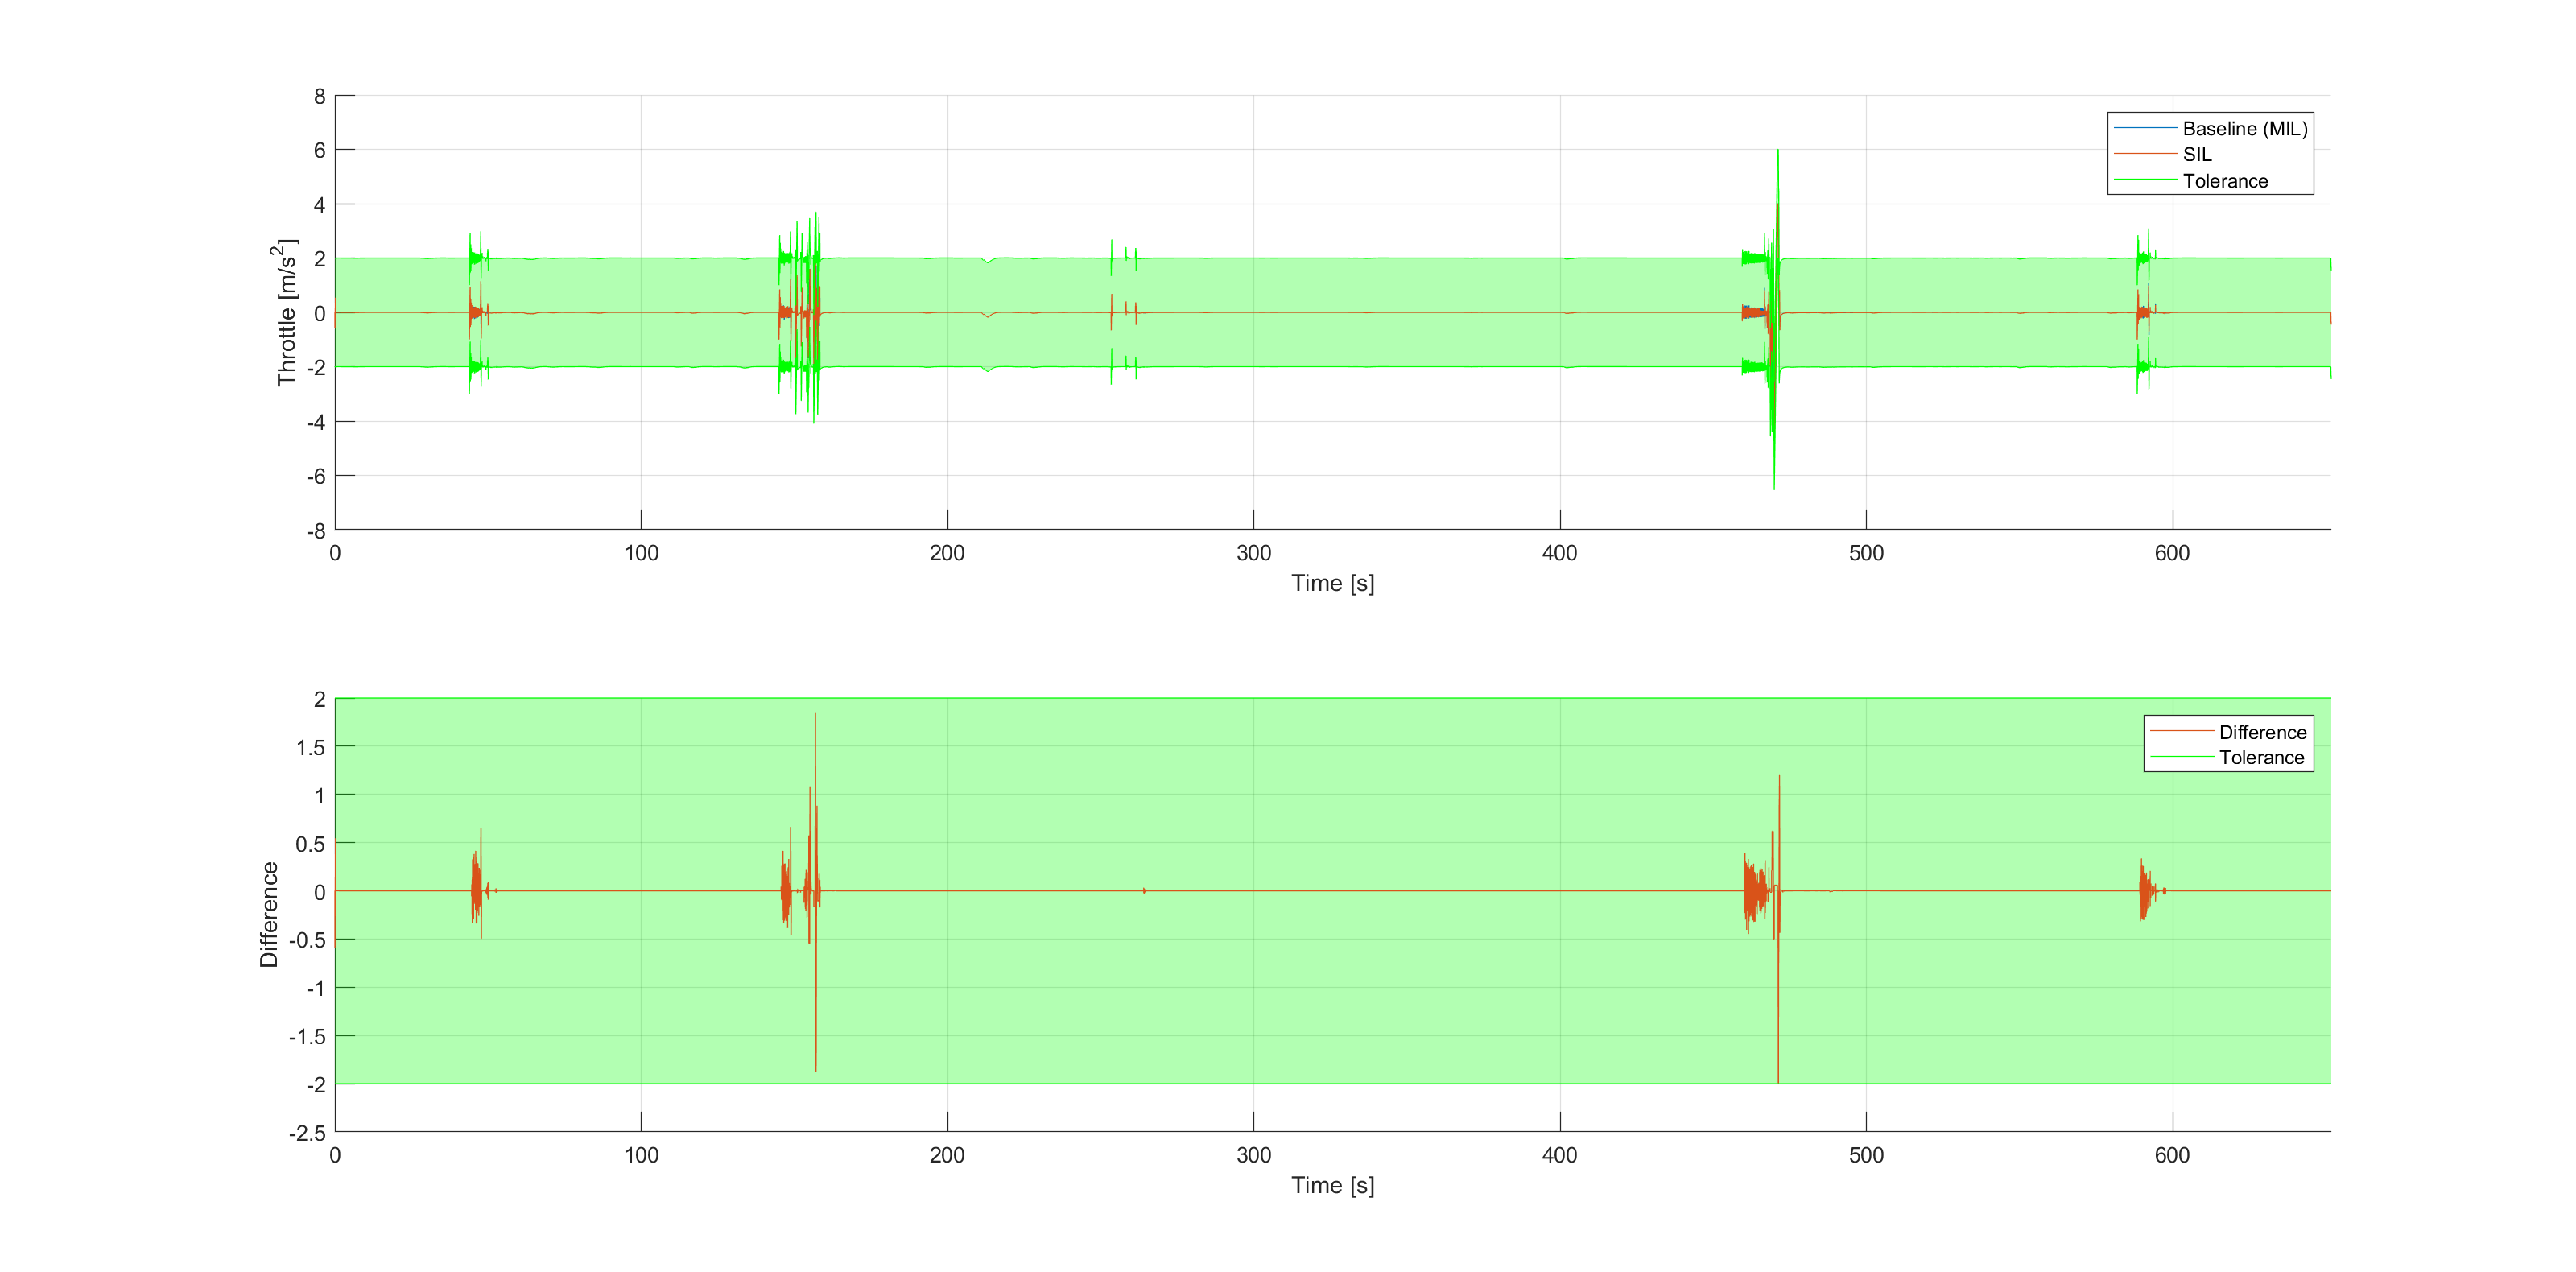
\includegraphics[width=1.1\textwidth,keepaspectratio]{Figures/throttle_volkswagen.png}
    \caption{Throttle deviations with Volkswagen Beetle in Puglia}
    \label{fig:throttle_beetle}
    \end{figure}%
    
In particular, in both the simulations with the Hyundai Azera and Ford E150, the exceeding deviation happened at the same point of the map, when the ego-car is passing the two consecutive static obstacles. Instead, in the simulation with the Volkswagen Beetle, the exceeding deviation happened when the ego-car is overtaking the first dynamic obstacle.\\
Before declaring the SIL a failure, it is important to highlight that we have not chosen carefully the tolerance values since our scope was to have a graphical representation of the deviation between the two simulations with some bounds. Moreover, as it is possible to recognize by the reports in the repository, the whole six assessments concerning the lateral deviation and lateral acceleration limits are totally verified in the SIL.





\subsection{PIL} \label{subsection:PIL}
For the Processor-in-the-Loop, the code generated is loaded into an external processor, usually a microcontroller, to evaluate the execution outcome on an architecture similar to the one where the final controller will be deployed.\\
For our project we had the availability of a STM32 Nucleo Board owned by one member of the team. Unfortunately, this board has only 64 kB of RAM while the code generated for the MPC needs more memory to be run as it is. Indeed, when trying to load the code on the board the building system returns an error.\\
As a solution, since the target of the project is to take confidence with the Model-Based Design technique, we have decided to generate only a part of the code for the PIL, in order to understand how to deal with this verification method.\\
The part of the code which we have chosen to generate and deploy on the controller is the ``Constraint Generator Function", that is the left block in Figure \ref{fig:simulink_mpc}, which takes as inputs the points and the flags generated by the obstacle detection function, and gives as outputs the constraint matrices E, F and G.\\
To deploy code on the Nucleo Board, we have used a Simulink extension (STM32-MAT) provided by ST-Microelectronics and some tools such as STM32CubeMX, to define the peripheral configuration, and STM32CubeIDE, to build the generated code and load it on the target board.\\
The Simulink model to run PIL test is depicted in Figure \ref{fig:PIL_Model}, where the top block (PIL\_Model) is the same of the bottom block (MIL\_Model), with the exception of the subsystem \textit{``Constraint Generator"}, which is modeled with a PIL block on the former and with a MATLAB function on the latter. The results of this test are the difference on the output states of the vehicle model.
\begin{figure}[H]
    \centering
    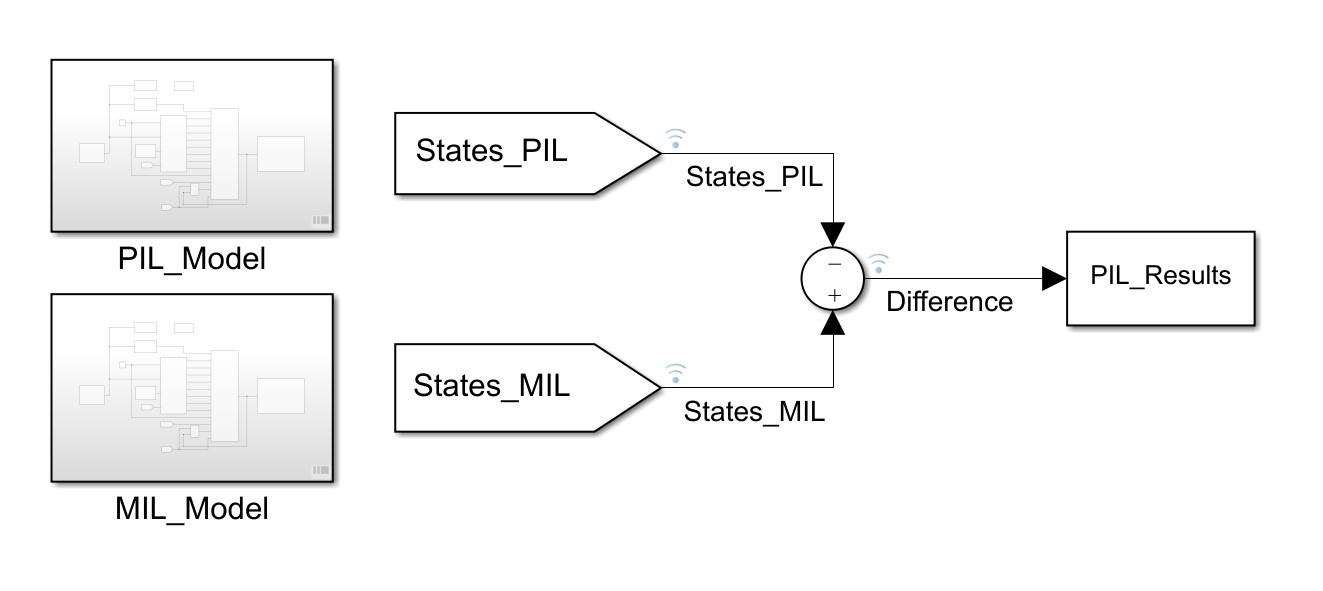
\includegraphics[width=1\textwidth,keepaspectratio]{Figures/PIL_Model.jpg}
    \caption{Simulation model for PIL}
    \label{fig:PIL_Model}
\end{figure}
We have decided to run this test on the same scenarios developed for MIL test, but we have run them only with vehicle 1 (Hyundai Azera) since PIL simulation requires a lot of time due to the serial communication between the Simulink environment and the MCU Board.\\
The results of this test are included in the Documentation folder\footnote{The ``PIL\_Test\_Reports"folder is included in the /Documentation/Test Reports/ file path.}. The difference between the model and the PIL is always null, probably because the function implemented on the MCU is very simple.
